%% LyX 2.0.6 created this file.  For more info, see http://www.lyx.org/.
%% Do not edit unless you really know what you are doing.
\documentclass[english,onecolumn]{elsarticle}
\usepackage[T1]{fontenc}
\usepackage[utf8]{inputenc}
\usepackage[a4paper]{geometry}
\geometry{verbose}
\usepackage{babel}
\usepackage{amsmath}
\usepackage{amssymb}
\usepackage{graphicx}
\usepackage{esint}
\usepackage[unicode=true]
 {hyperref}

\makeatletter
%%%%%%%%%%%%%%%%%%%%%%%%%%%%%% User specified LaTeX commands.
%\@ifundefined{definecolor}
% {\usepackage{color}}{}
%\makeatother

%\makeatother


\usepackage{times}
%\usepackage{subfloat}
%\usepackage{subfig}
\usepackage{psfrag}
\usepackage{babel}
\usepackage{times}


%%%
\makeatletter
\def\ps@pprintTitle{%
  \let\@oddhead\@empty
  \let\@evenhead\@empty
  \def\@oddfoot{\reset@font\hfil\thepage\hfil}
  \let\@evenfoot\@oddfoot
}
\makeatother

\makeatother

\begin{document}

\title{T'aurais pas une entropie?}


\author{by jfb \& co \date}
\begin{abstract}
Where we show that it is possible to derive new entropies yielding
a particular specified maximum entropy distribution. There are (probably)
many errors --I hope not fundamental but is is possible; (certainly
many) approximations, typos, maths and language mistakes.Suggestions
and improvements will be much appreciated. 
\end{abstract}
\maketitle

\section{Maximum entropy distributions}

Let $S[f]=\int f(x)\log f(x)\mathrm{d}\mu(x)$ be the Shannon entropy.
Subject to on, or several moment constraints such as $\mathbb{E}[T_{i}(x)]=m_{i},$
and to normalization, it is well known that the maximum entropy distribution
lies within the exponential family 
\[
f_{X}(x)=\exp\left(\sum_{i}\lambda_{i}T_{i}(x)+\mu\right).
\]
In order to recover known probability distributions (that must belong
to the exponential family), it is then sufficient to specify a function
$T(x).$ This has been used by many authors. For instance, the gamma
distribution can be viewed as a maximum entropy distribution if one
knows the moments $\mathbb{E}[X]$ and $\mathbb{E}[\log(X)].$ In
order to find maximum entropy distributions with simpler constraints
or distributions outside of the exponential family, it is possible
to consider other entropies. This is discussed below. 


\section{Maximum $(h,\phi)$-entropy distributions}


\subsection{Definition and maximum $(h,\phi)$-entropy solution}

\global\long\def\dmu#1{\mathrm{d}\mu(#1)}


Let us consider a convex function $\phi(x)$ and define a $\phi$-entropy
as 
\begin{equation}
H_{\phi}[f]=\int\phi(f(x))\mathrm{d}\mu(x)\label{eq:phi-entropy}
\end{equation}
If $\phi(x)$ is convex, then so is the entropy functional $H_{\phi}[f]$.
Also note that the composition with a convex non decreasing function
preserves convexity, and that composition with a concave non increasing
function yields a concave functional, thus yielding the $(h,\phi)$-entropy
functional 

\begin{equation}
H_{h,\phi}[f]=h\left(\int\phi(f(x))\mathrm{d}\mu(x)\right)\label{eq:h-phi-entropy}
\end{equation}


Consider the maximum entropy problem subject to a constraint on some
moment $\mathbb{E}\left[T(X)\right]$. Since $h$ is assumed monotone,
it is enough to look for the minimum of the $\phi$-entropy (\ref{eq:phi-entropy}):
\[
\begin{cases}
\max_{f} & -\int\phi(f(x))\mathrm{d}\mu(x)\\
\text{s.t. } & \mathbb{E}\left[T(X)\right]=m\\
\text{and} & \mathbb{E}\left[1\right]=1
\end{cases}
\]


For now, let us use the classical Lagrange multipliers technique.
We will give another proof of the result later. The Lagrangian is
\[
L(f;\lambda,\mu)=-\int\phi(f(x))\mathrm{d}\mu(x)+\lambda\int T(x)f(x)\dmu x+\mu\left(\int f(x)\dmu x\right),
\]
where the parameter $\lambda$ enables to satisfy th emoment constraint
while $\mu$ is associated with the normalization constraint. The
stationnary points statisfy the Euler-Lagrange equation
\[
\phi'(f(x))+\lambda T(x)+\mu=0
\]
which gives 
\begin{equation}
f_{X}(x)=\phi'^{-1}\left(\lambda T(x)+\mu\right).\label{eq:sol-h-phi}
\end{equation}


An alternative derivation of the result consists in checking that
the distribution (\ref{eq:sol-h-phi}) is effectively a maximum entropy
distribution, by showing that $H_{\phi}[f]>H_{\phi}[g]$ for all probability
distributions with a given (fixed) moment $\mathbb{E}\left[T(X)\right].$
The Bregman divergence associated with $\phi$ defined on a closed
convex set $\Omega,$ is given by
\[
D_{\phi}(x_{1},x_{2})=\phi(x_{1})-\phi(x_{2})-\phi'(x_{2})\left(x_{1}-x_{2}\right).
\]
As is well known, the Bregman divergence is nonegative $D_{\phi}(x_{1},x_{2})\geq0\,\,\forall x_{1},x_{2}\in\Omega,$
with equality if and only if $x_{1}=x_{2}.$ A functional Bregman
divergence can be defined for a convex function acting on functions:
\[
D_{\phi}(f_{1},f_{2})=\int\phi(f_{1})\mathrm{d}\mu(x)-\int\phi(f_{2})\mathrm{d}\mu(x)-\int\phi'(f_{2})\left(f_{1}-f_{2}\right)\mathrm{d}\mu(x).
\]
This divergnce is nonnegative as well, and zero if and only if $f_{1}(x)=f_{2}(x)$\,\,$\forall x$.
Define by 
\[
C=\left\{ f:\,\,\, f\geq0,\mathbb{\,\,\,\, E}\left[1\right]=1,\mathbb{\,\, E}\left[T(X)\right]=t\right\} 
\]
the set of all probability distributions with a given moment. Let
now $f_{2}(x)\in C,$ with $f_{2}(x)=\phi'^{-1}\left(\lambda T(x)+\mu\right)$.
Now consider $f_{1}\in C$, then 
\begin{alignat}{1}
D_{\phi}(f_{1},f_{2}) & =\int\phi(f_{1})\mathrm{d}\mu(x)-\int\phi(f_{2})\mathrm{d}\mu(x)-\int\phi'(f_{2})\left(f_{1}-f_{2}\right)\mathrm{d}\mu(x)\\
 & =\int\phi(f_{1})\mathrm{d}\mu(x)-\int\phi(f_{2})\mathrm{d}\mu(x)-\int\phi'(\phi'^{-1}\left(\lambda T(x)+\mu\right))\left(f_{1}-f_{2}\right)\mathrm{d}\mu(x)\\
 & =\int\phi(f_{1})\mathrm{d}\mu(x)-\int\phi(f_{2})\mathrm{d}\mu(x)-\int\left(\lambda T(x)+\mu\right)\left(f_{1}-f_{2}\right)\mathrm{d}\mu(x)\label{eq:before_simp}\\
 & =H_{\phi}[f_{1}]-H_{\phi}[f_{2}]\label{eq:after_simp}
\end{alignat}
where we used in (\ref{eq:before_simp}) the fact that $f_{1}$and
$f_{2}$ are normalized to one and have the same moment $\mathbb{E}\left[T(X)\right]$.
By nonegativity of the Breman fuctional divergence, we finally get
that 
\[
H_{\phi}[f_{1}]\geq H_{\phi}[f_{2}]
\]
for all pdf with a given moment, with equality if and only if $f_{1}=f_{2}.$
In other words, this sows that (\ref{eq:sol-h-phi}) realizes the
minimum of $H_{\phi}[f].$


\subsection{Defining new entropy functionals}

Given an entropy functional, we thus obtain a maximum entropy distribution.
There exists numerous $(h,\phi)$-entropies in the literature. However
a few of them lead to explicit forms for the maximum entropy distribution.
Therefore, it is of high interest to look for the entropies that lead
to a specified distribution as a maximum entropy solution. 

Let $f_{X}(x)$ be a probability distribution. We may consider the
whole family associated with scale and translation transformations,
that is $x\rightarrow\left(x-x_{0}\right)/\sigma,$ with density $\frac{1}{\sigma}f_{X}\left(\frac{x-x_{0}}{\sigma}\right).$
Since we have to equate this density to $\phi'^{-1}\left(\lambda T(x)+\mu\right)$,
we see that $\lambda$ plays the role of the precision parameter and
$\mu$ of the location parameter. 

Since we will look for the function $\phi$ for a given probability
distribution $f_{X}(x)$ we also see that the corresponding $(\lambda,\mu)$
parameters can be included in the definition of the function. 

It is thus enough to restrict ourselves to the case $(\lambda=1,\mu=0),$
and look for $\phi(x)$ such that 
\begin{equation}
\phi'^{-1}\left(\lambda T(x)+\mu\right)=f_{X}(x).\label{eq:aresoudre}
\end{equation}


Let us recall some implicit properties of $\phi(x).$ 
\begin{itemize}
\item $\phi''(x)\geq0$, since $\phi(x)$ is assumed convex. This also means
that $\phi'(x)$ is non decreasing,
\item $\phi'(x)$ is defined on $[0,$$\sup_{x}f(x)]$. 
\end{itemize}
The identification of a function $\phi(x)$ such that a given $f_{X}(x)$
is the associated maximum entropy distribution amounts to solve (\ref{eq:aresoudre}),
that is 
\begin{enumerate}
\item choose $T(x)$,
\item find $\phi'(y)$ such that 
\begin{equation}
\lambda T(x)+\mu=\phi'\left(f_{X}(x)\right)=\phi'(y)\label{eq:inv}
\end{equation}

\item integrate the result to get $\phi(y)=\int\phi'(y)dy+c$, where $c$
is an integration constant. The entropy being defined by $H_{\phi}[f]=\int\phi(f(x)\,\text{d}\mu(x)$,
the constant $c$ will usually be zero. 
\item The parameters $\lambda$ and $\mu$ may be choosen case by case in
order to simplify the expression of $\phi.$ 
\end{enumerate}
Observe that since we want $\phi(x)$ to be convex, which means $\phi''(x)\geq0$
for a twice differeentiable function, it is thus necessary that $\phi'(x)$
is non decreasing on $[0,$max$(f)]$. By (\ref{eq:aresoudre}), we
have that 
\[
f_{X}'(x)=\lambda T'(x)\frac{1}{\phi''\left(\phi'^{-1}\left(\lambda T(x)+\mu\right)\right)}=\lambda T'(x)\frac{1}{\phi''\left(f_{X}(x)\right)}.
\]
Hence we get that 
\[
\phi''\left(f_{X}(x)\right)=\frac{f_{X}'(x)}{\lambda T'(x)}
\]
and we see that $f_{x}(x)$ and $T(x)$ must have the same or an opposite
variation, depending on the sign of $\lambda$. 

Examples: if $\lambda$ is negative, then 
\begin{itemize}
\item for $T(x)=x,$ $f_{X}(x)$ must be non increasing,
\item for $T(x)=x^{2}$ or $T(x)=|x|,$ $f_{X}(x)$ must be unimodal with
a maximum at zero. 
\end{itemize}
Let us consider some specific cases. 
\begin{enumerate}
\item For a normal distribution, $f_{X}(x)=\frac{1}{\sqrt{2\pi}}\exp(-\frac{x^{2}}{2})$
and $T(x)=x^{2},$ we begin by computing the inverse $y=\frac{1}{\sqrt{2\pi}}\exp(-\frac{x^{2}}{2})$,
which gives $-\frac{1}{2}x^{2}-\log\sqrt{2\pi}=\log(y).$ Choosing
$\lambda=-\frac{1}{2}$, $\mu=-\log\sqrt{2\pi}$ and integrating,
we obtain 
\[
\phi(y)=y\log y-y
\]

\item For a Tsallis $q$-exponential, $f_{X}(x)=C_{q}\left(1-(q-1)\beta x\right)_{+}^{\frac{1}{(q-1)}},$
$x\geq0,$ and $T(x)=x$. We simply have $C_{q}^{q-1}\left(1-(q-1)\beta x\right)=y^{q-1}$.
With $\lambda=qC_{q}^{q-1}\beta$ and $\mu=qC_{q}^{q-1}/(1-q)$, this
yields 
\[
\phi(y)=\frac{y^{q}}{1-q}.
\]
Taking $\mu=\left(qC_{q}^{q-1}+1\right)/(1-q)$ gives 
\[
\phi(y)=\frac{y^{q}-y}{1-q},
\]
and an associated entropy can be 
\[
H_{\phi}[f]=\frac{1}{1-q}\left(\int f(x)^{q}\text{d}\mu(x)-1\right),
\]
which is nothing but Tsallis entropy.%
\footnote{Of course, we can also take the first $\phi(y)=\frac{y^{q}}{1-q},$
integrate and add any constant, since adding a constant do not modify
the actual value af the minimizer (or maximizer if we consider concave
entropies). %
}
\item The same entropy functional can readily be obtained for the so-called
$q$-Gaussian, or Student-t and -r distributions $f_{X}(x)=C_{q}\left(1-(q-1)\beta x^{2}\right)_{+}^{\frac{1}{(q-1)}}.$
It suffices to follow the very same steps as above with $T(x)=x^{2}.$ 
\item Let $f_{X}(x)$ be the hyperbolic secant distribution, with density
\[
f_{X}(x)=\frac{1}{2}\text{sech}(\frac{\pi}{2}x)=\frac{1}{2}\cosh^{-1}(\frac{\pi}{2}x).
\]
Obviously, $\frac{\pi}{2}x=\cosh(2y)=\phi'(y)$ with $T(x)=x$, $\lambda=\frac{\pi}{2}$,
and 
\[
\phi(y)=\sinh(2y).
\]
So doing, we obtain an hyperbolic sine entropy with the hyperbolic
secant distribution as the associated maximum entropy distribution.
\end{enumerate}
Of course, the preceeding derivations require that (\ref{eq:inv})
is effectively solvable. Furthermore, one has also to choose or design
a specific $T(x)$ statistic, as well as the parameters $\lambda$
and $\mu$. In the examples above, we used $T(x)=x$ and $T(x)=x^{2}.$
Particular choices such as $T(x)=x^{2}$ or $T(x)=|x|$ obviously
lead to symmetrical densities. The case of nonsymmetrical unimodal
densities seems to be much more involved. For instance, if we take
$T(x)=x$, then the resolution of (\ref{eq:inv}) amounts to compute
the inverse relation of $f_{X}(x)$, which is is multi-valued. We
will deal now with this special case. 


\subsection{Entropies for unimodal nonsymmetric distributions}

Assume, without loss of generality that the mode is $x=0.$ Let $T(x)=x$,
and $\lambda=-1$, $\mu=0.$ In such case, we have to find $\phi$
satisfying $x=-\phi'\left(f_{X}(x)\right)=-\phi'(y)$. We see that
$\phi'$ is minus the inverse relation of $y=f_{X}(x)$. But $f_{X}(x)$
is not injective and to each $y$ correspond a positive and a negative
value of $x.$ Hence we have two partial inverses, say $\phi_{+}'$
and $\phi_{-}'$ such that $\phi_{+}'^{-1}(-x)=f_{X}(x)$ for $x\geq0$
and $\phi_{-}'^{-1}(-x)=f_{X}(x)$ for $x\leq0$. We observed above
that if $f_{X}(x)$ is non increasing, that is assumed here for $x\geq0,$
then $\phi_{+}''\geq0$ and $\phi_{+}$is convex. Then, our proposal
is to use the functional $\phi_{+}$ for defining a $\phi$-entropy
\[
H_{\phi}[f_{X}]=\int\phi_{+}\left(f_{X}(x)\right)\dmu x
\]
associated with a specific nonsymmetric probability distribution.
In this setting, it is understood that the maximum entropy distribution
$f_{X}(x)=\phi'^{-1}(-x)$ will have to be computed as $\phi_{+}'^{-1}(-x)=f_{X}(x)$
for $x\geq0$ and $\phi_{-}'^{-1}(-x)=f_{X}(x)$ for $x\leq0$. Of
course, this does not forbid to model one-sided probability distribution,
provided that the constraint is included in the formulation of the
maximum entropy problem. 


\subsubsection{Example 1. The logistic distribution}

The pdf of the logistic distribution is given by
\[
f_{X}(x)=\frac{e^{-\frac{x}{s}}}{s\left(1+e^{-\frac{x}{s}}\right)^{2}}.
\]
This distribution, which resembles the normal distribution but has
heavier tails, has been used in many applications. By direct calculations,
we obtain 
\[
\begin{cases}
\phi_{-}'(y)= & s\ln\left(\frac{1}{2}\,{\frac{-2\, ys+1+\sqrt{-4\, ys+1}}{ys}}\right),\\
\phi_{+}'(y)= & s\ln\left(-\frac{1}{2}\,{\frac{2\, ys-1+\sqrt{-4\, ys+1}}{ys}}\right).
\end{cases}
\]


The associated entropy is then 
\[
\phi_{+}(y)=\frac{1}{2}\,\sqrt{-4\, ys+1}+ys\,\ln\left(-{\frac{\sqrt{-4\, ys+1}-1}{\sqrt{-4\, ys+1}+1}}\right),
\]
for $y\in[0,\frac{1}{4s}],$ and where we have introduced a integration
constant such that $\min_{y}\phi_{+}(y)=0.$ For $y>\frac{1}{4s},$
we extend the function and let $\phi_{+}(y)=+\infty.$ Figure \ref{fig:Entropy-logistic}
\begin{figure}
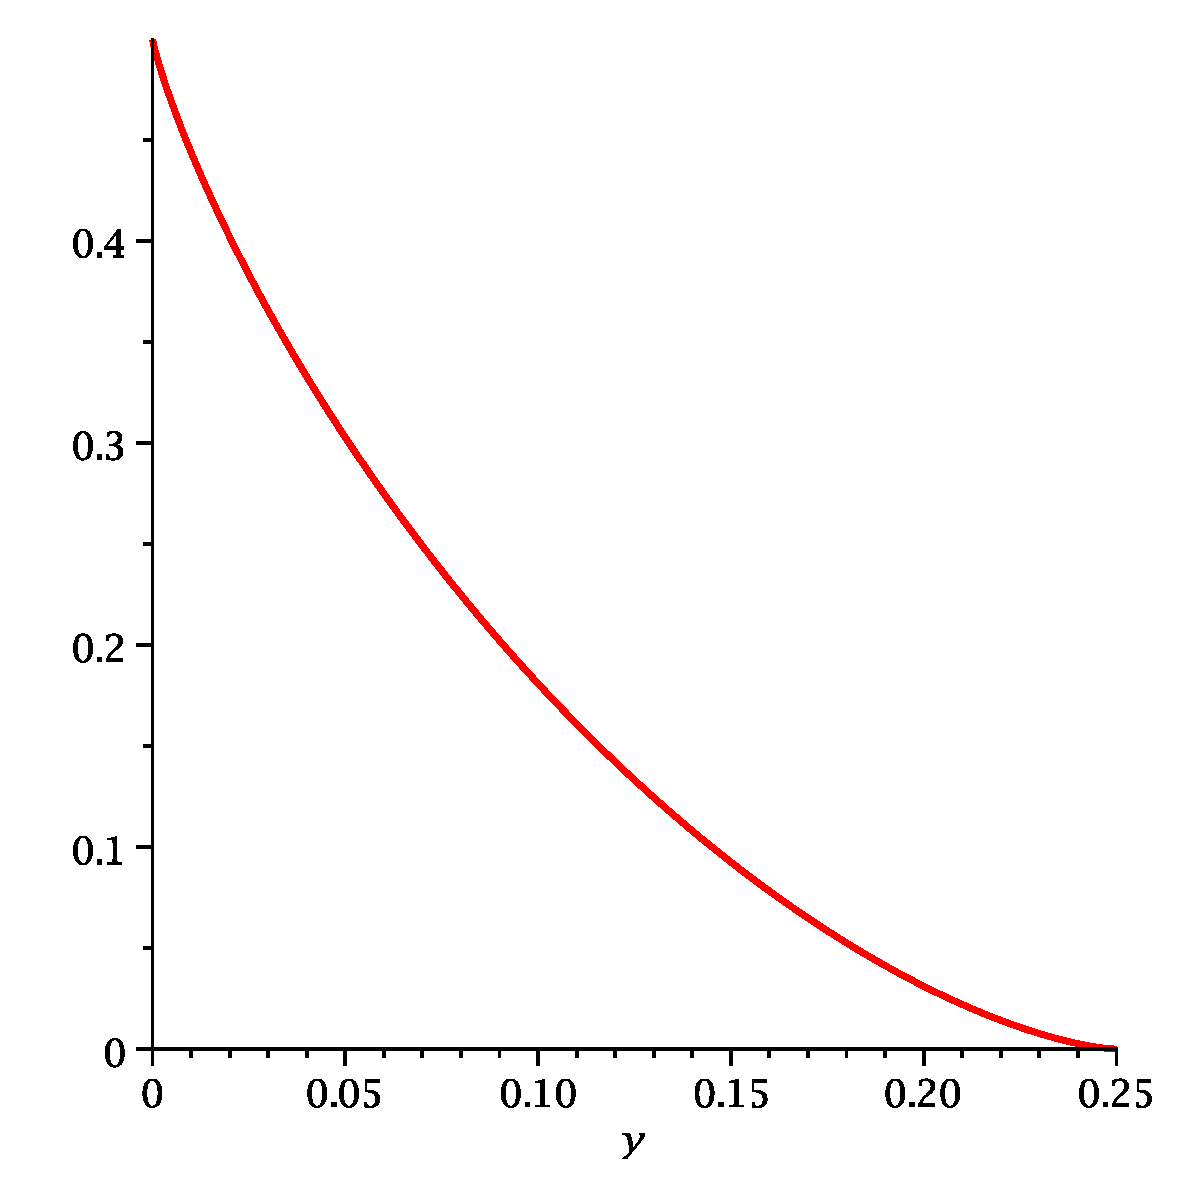
\includegraphics[width=5cm]{maple/phi_logistic}\caption{Entropy derived from the logistic distribution. \label{fig:Entropy-logistic}}


\end{figure}
gives a representation of this entropy for $s=1.$ 


\subsubsection{Example 2. The gamma distribution}

The probability density function of the gamma distribution is given
by 
\[
f_{X}(x)=\frac{{\beta}^{\alpha}{x}^{\alpha-1}{e}^{-\beta\, x}}{\Gamma\left(\alpha\right)}
\]


We obtain 
\[
\phi'(y)=-{{\rm e}^{\frac{1}{\alpha-1}\left(-{\it W}\left(-{\frac{\beta\,\left(y\Gamma\left(\alpha\right){\beta}^{-\alpha}\right)^{\left(\alpha-1\right)^{-1}}}{\alpha-1}}\right)\alpha+{\it W}\left(-{\frac{\beta\,\left(y\Gamma\left(\alpha\right){\beta}^{-\alpha}\right)^{\left(\alpha-1\right)^{-1}}}{\alpha-1}}\right)+\ln\left(y\Gamma\left(\alpha\right){\beta}^{-\alpha}\right)\right)}},
\]
where ${\it W}$ is the Lambert W multivalued `function' defined by
$z=W(z)e^{W(z)}$ (ie the inverse relation of $f(w)=we^{w}$). Unfortunately,
in the general case, we do not have a closed form for $\phi(y)$ as
the integral of $\phi'(y)$.%
\footnote{This might not be completely unacceptable. Indeed, it is really not
difficult to compute numerically the values of $\phi(y).$%
} Restricting us to the case $\alpha=2$, we have
\[
\phi(y)=\frac{\left(1-{\it W}\left(-{\frac{y}{\beta}}\right)+y\left({\it W}\left(-{\frac{y}{\beta}}\right)\right)^{2}\right)}{{\it \beta\, W}\left(-{\frac{y}{\beta}}\right)}+\frac{\beta}{e},
\]
which is convex if we choose the -1 branch of the Lambert function.
An example with $\alpha=2$ and $\beta=3$ is given on Figure \ref{fig:Entropy-gamma}.
\begin{figure}
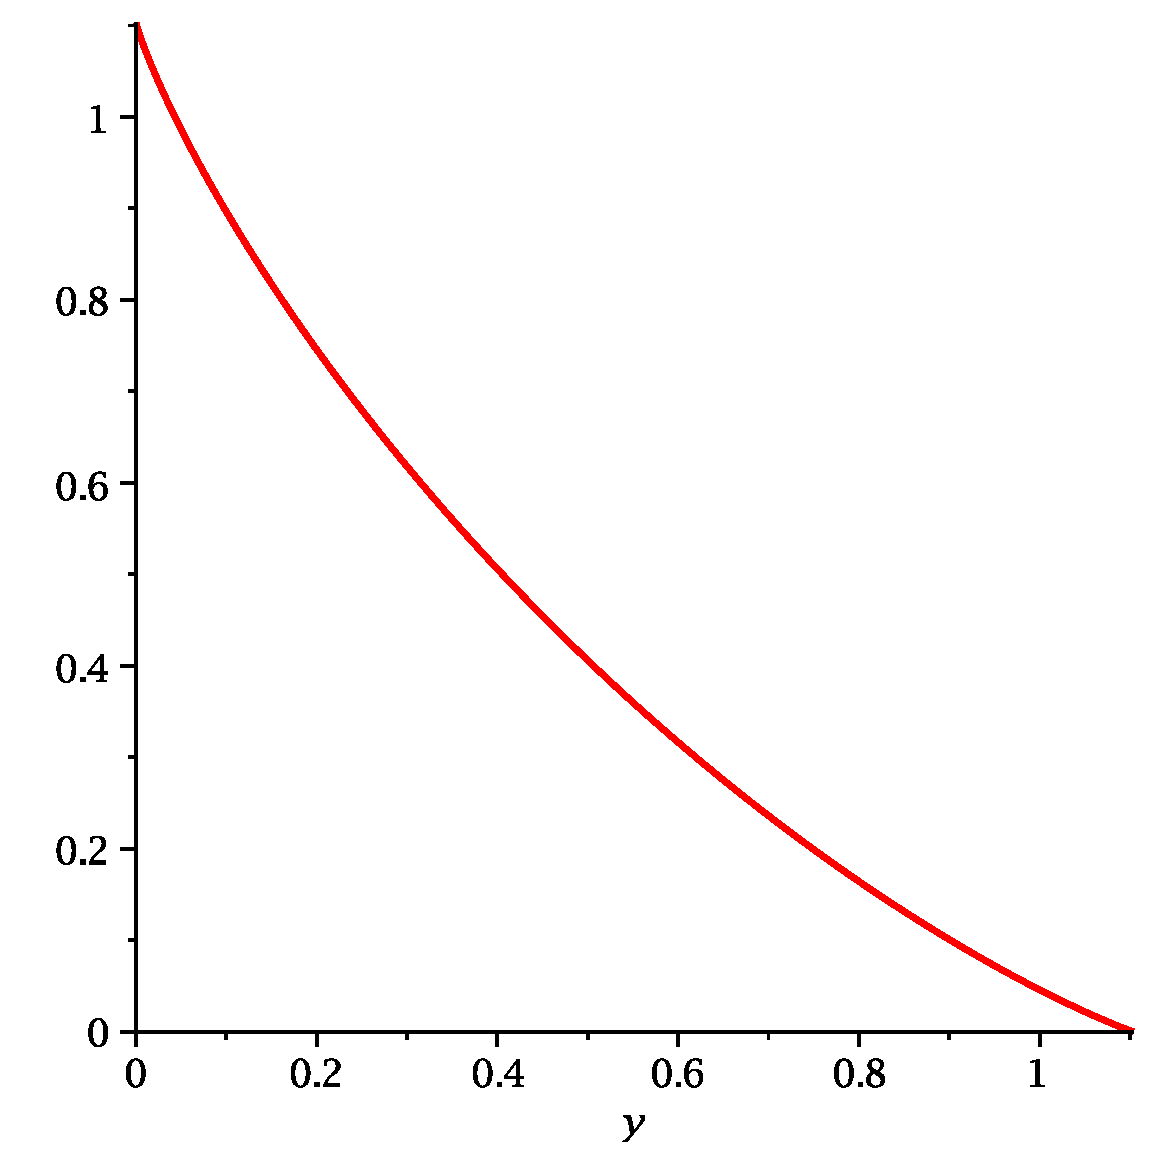
\includegraphics[width=5cm]{maple/phi_gamma}\caption{\label{fig:Entropy-gamma}Entropy derived from the gamma distribution}
\end{figure}



\subsubsection{Example 3. The arcsine distribution}

As a last example, and though it is not a unimodal density (! but
yields the same problem for inversion), let us consider the case of
the arcsine distribution (see \href{http://en.wikipedia.org/wiki/Arcsine_distribution}{wiki}).
This distribution, defined for $x\in(0,1),$ is a special case of
the Beta distribution with parameters $\alpha=\beta=1/2.$ It has
the following pdf:
\[
f_{X}(x)=\frac{1}{\pi\sqrt{x(1-x)}}.
\]
Observe that $\min_{x}f_{X}(x)=2/\pi.$ Doing our now usual calculations,
we obtain
\[
\begin{cases}
\phi_{-}'(y)= & -\frac{\, y\pi+\,\sqrt{{y}^{2}{\pi}^{2}-4}}{2y\pi},\\
\phi_{+}'(y)= & -\frac{\, y\pi-\,\sqrt{{y}^{2}{\pi}^{2}-4}}{2y\pi}.
\end{cases}
\]
and the expression of the entropy is 
\[
\phi_{+}(y)=\frac{1}{2}\,{\frac{\sqrt{{y}^{2}{\pi}^{2}-4}}{\pi}}+\frac{1}{\pi}\arctan\left(2\,{\frac{1}{\sqrt{{y}^{2}{\pi}^{2}-4}}}\right)-\frac{1}{2}\, y,
\]
for $y\geq1/\pi$. The entropy is shown on Figure \ref{fig:arcseine entropy}.
\begin{figure}
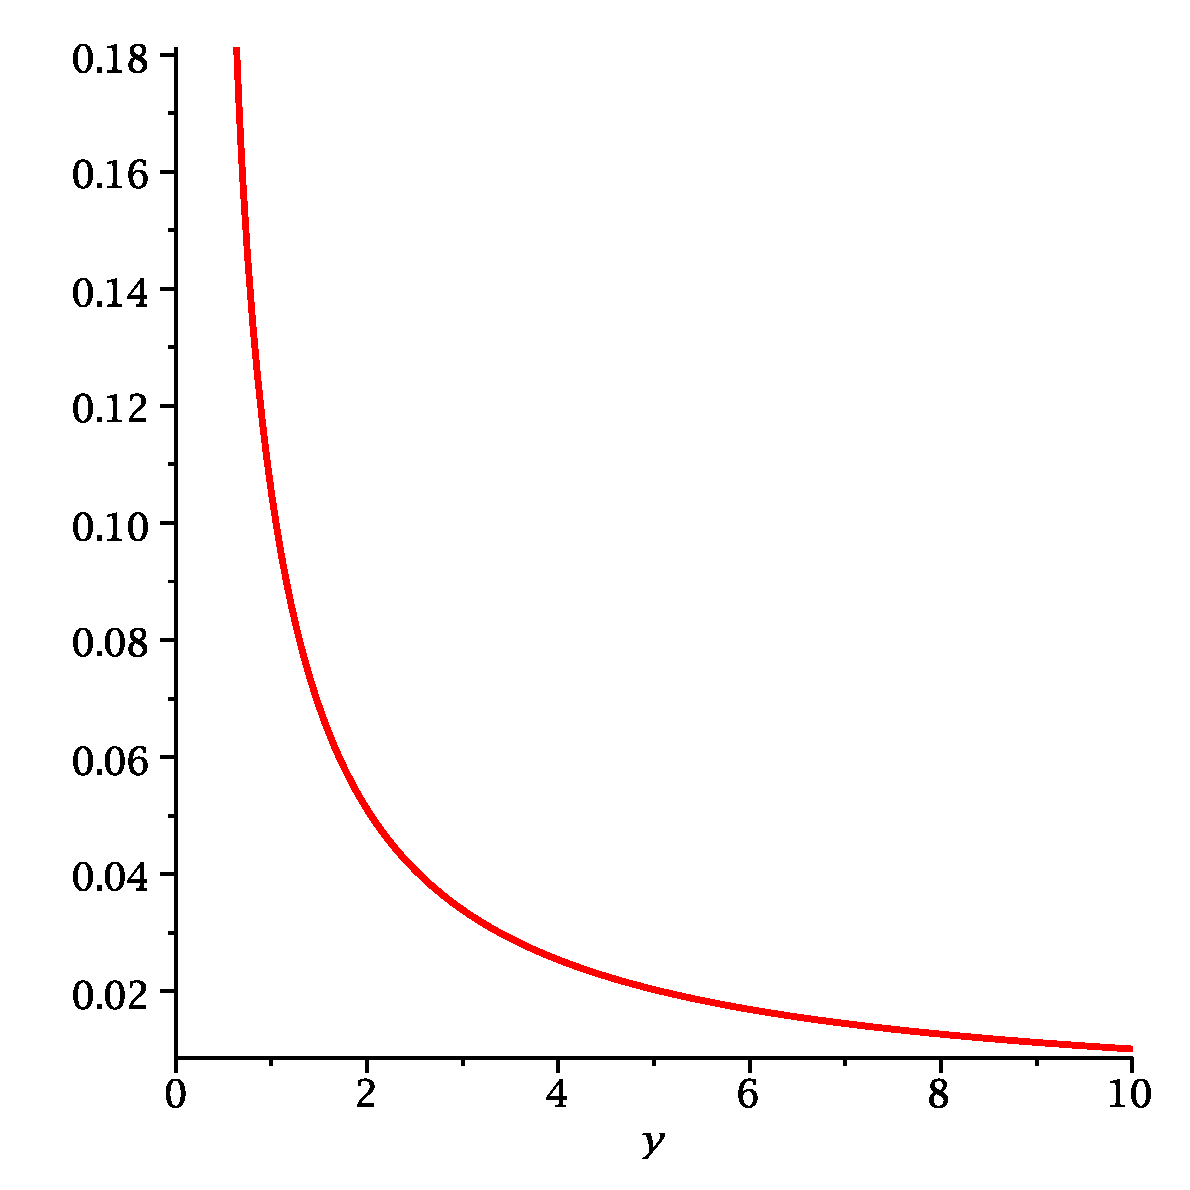
\includegraphics[width=5cm]{maple/phi_arcsine}\caption{The entropy associated with an arcsine distribution. \label{fig:arcseine entropy}}


\end{figure}

\end{document}
